\documentclass[utf8x,xcolor=pdftex,dvipsnames,table]{beamer}
\usetheme{Malmoe}  % Now it's a beamer presentation with the lisa theme!
\setbeamertemplate{footline}[page number]
\usecolortheme{beaver}
\usepackage[T1]{fontenc}
\usepackage{amsmath}
\usepackage[utf8x]{inputenc}
%\logo{\includegraphics[width=.8in]{UdeM_NoirBleu_logo_Marie_crop}}
\usepackage{listings}

\newcommand{\superscript}[1]{\ensuremath{^{\textrm{#1}}}}

\mode<presentation>

\title{Theano, Pylearn2, libgpuarray Presentation}

\author{%
\footnotesize
Frédéric Bastien, Bart van Merriënboer \newline
Département d'Informatique et de Recherche Opérationnelle \newline
Université de Montréal \newline
Montréal, Canada \newline
\texttt{\{bastienf, vanmerb\}@iro.umontreal.ca} \newline \newline
}

\date{OML Workshop 2014}

\setbeamertemplate{navigation symbols}{}

\begin{document}

\begin{frame}[plain]
 \titlepage
 \vspace{-5em}
 \includegraphics[width=1in]{../hpcs2011_tutorial/pics/lisabook_logo_text_3.png}
 \hfill
 \includegraphics[width=.8in]{../hpcs2011_tutorial/pics/UdeM_NoirBleu_logo_Marie_crop}
\end{frame}

\section{Introduction}
\begin{frame}{High level}\setcounter{page}{1}
  Python <- \{NumPy/SciPy/libgpuarray\} <- Theano <- Pylearn2
  \begin{itemize}
  \item Python: OO coding language
  \item Numpy: $n$-dimensional array object and scientific computing toolbox
  \item SciPy: sparse matrix objects and more scientific computing functionality
  \item libgpuarray: GPU $n$-dimensional array object in C for CUDA and OpenCL
  \item Theano: compiler/symbolic graph manipulation
  \item Pylearn2: machine learning framework
  \end{itemize}
\end{frame}


%% \begin{frame}{Others}
%%   \begin{itemize}
%%   \item matplotlib: one of the many plotting library
%%   \item IPython: Advanced python shell
%%   \item IPython notebook: web-based interactive computational environment where you can combine code execution, text, mathematics, plots and rich media into a single document
%%   \end{itemize}
%% \end{frame}

\begin{frame}{Python}
  \begin{itemize}
  \item General-purpose high-level OO interpreted language
  \item Emphasizes code readability
  \item Comprehensive standard library
  \item Dynamic type and memory management
  \item Slow execution
  \item Easily extensible with C
  \item Popular in {\em web development}\ and {\em scientific communities}
  \end{itemize}
\end{frame}

\begin{frame}{NumPy/SciPy}
  \begin{itemize}
  \item Python floats are full-fledged objects on the heap
      \begin{itemize}
      \item Not suitable for high-performance computing!
      \end{itemize}

  \item NumPy provides an $n$-dimensional numeric array in Python
      \begin{itemize}
      \item Perfect for high-performance computing
      \item Slices of arrays are views (no copying)
      \end{itemize}

  \item NumPy provides
      \begin{itemize}
      \item Elementwise computations
      \item Linear algebra, Fourier transforms
      \item Pseudorandom number generators (many distributions)
      \end{itemize}

  \item SciPy provides lots more, including
      \begin{itemize}
      \item Sparse matrices
      \item More linear algebra
      \item Solvers and optimization algorithms
      \item Matlab-compatible I/O
      \item I/O and signal processing for images and audio
      \end{itemize}
  \end{itemize}
\end{frame}

\begin{frame}{What's missing?}
  \begin{itemize}
    \item Non-lazy evaluation (required by Python) hurts performance
    \item Bound to the CPU
    \item Lacks symbolic or automatic differentiation
    \item No automatic speed and stability optimization
  \end{itemize}

\end{frame}

%% \begin{frame}{Why scripting for GPUs?}
%%   \begin{bf}They complement each other\end{bf}

%%   GPUs are everything that high level languages are not

%%   \begin{itemize}
%%     \item Highly parallel
%%     \item Very architecture-sensitive
%%     \item Built for maximum FP/memory throughput
%%     \item So hard to program that meta-programming is easier
%%   \end{itemize}

%%   \begin{bf}Best of both worlds:\end{bf} easily scripted code which invokes high-performance GPU kernels.

%%   \begin{bf}Theano C code generation removes overhead\end{bf} of
%%   function calls between Python and C by launching many C functions at once.

%% \end{frame}

\begin{frame}{Theano}

  High-level domain-specific language tailored to numeric computation.

  \begin{itemize}
    \item Syntax as close to NumPy as possible
    \item Compiles most common expressions to C for CPU and/or GPU
    \item Limited expressivity means more opportunities optimizations
    \begin{itemize}
      \item No subroutines -> global optimization
      \item Strongly typed -> compiles to C
      \item Array oriented -> easy parallelism
      \item Support for looping and branching in expressions
    \end{itemize}
    \item Automatic speed and stability optimizations
    \item Can reuse other technologies for best performance.
    \begin{itemize}
      \item BLAS, SciPy, Cython, Numba, PyCUDA, CUDA
    \end{itemize}
    \item Automatic differentiation and R op
    \item Sparse matrices
  \end{itemize}
\end{frame}


\begin{frame}{Pylearn2}

  Machine Learning library aimed at researchers

  \begin{itemize}
    \item Built on top of Theano, for fast execution and use of GPU
    \item Easy to try variants of implemented algorithms, and to extend them (using Theano)
    \item Very modular, each component of the library can be used in isolation
    \item Experiments can be specified through a YAML config file, or by a Python script
    \item Scripts for visualizing weights, plot monitored values
  \end{itemize}
\end{frame}


\begin{frame}{libgpuarray}
  Goal: A common GPU $n$-dimensional array that can be reused by all projects, support for both CUDA and OpenCL.
  \newline \newline
  Motivation:
  \begin{itemize}
  \item Currently there are at least 6 different GPU arrays in Python
    \begin{itemize}
    \item CudaNdarray (Theano), GPUArray (pycuda), CUDAMatrix (cudamat), GPUArray (pyopencl), Clyther, Copperhead, ...
    \item There are even more if we include other languages.
    \end{itemize}
  \item They are incompatible
    \begin{itemize}
    \item None have the same properties and interface
    \end{itemize}
  \item All of them implement a subset of numpy.ndarray properties
  \item This is the new GPU backend on Theano
  \end{itemize}
\end{frame}


\begin{frame}{Goal of the stack}
\begin{center}
\begin{bf}Fast to develop\end{bf}\newline \bigskip
\begin{bf}Fast to run\end{bf}\newline \bigskip


\includegraphics[width=0.35\textwidth]{road-runner-1.jpg}
\end{center}
\end{frame}


\section{Theano}
% I think it is a good idea to make explicit the change into a new section -- PL
\begin{frame}
  \tableofcontents[currentsection]
\end{frame}

\begin{frame}{Description}
  \begin{itemize}
    \item Mathematical symbolic expression compiler
    \item Expressions mimic NumPy's syntax and semantics
    \item Dynamic C/CUDA code generation
    \begin{itemize}
      \item C/C++, CUDA, OpenCL, PyCUDA, Cython, Numba, \ldots
    \end{itemize}
    \item Efficient symbolic differentiation
    %\begin{itemize}
    %  \item Derivatives of functions with one or many inputs.
    %  \item Computation of the Jacobian, Hessian, R and L op.
    %\end{itemize}
    \item Speed and stability optimizations
    \begin{itemize}
      \item Gives the right answer for ``$\log (1 + x)$'' even if $x$ is really tiny.
    \end{itemize}
    \item Extensive unit-testing and self-verification
    %\begin{itemize}
    %  \item Detects and diagnoses many types of errors
    %\end{itemize}
    \item Works on Linux, OS X and Windows
    \item Transparent use of a GPU
    \begin{itemize}
      \item {\tt float32} only for now (libgpuarray provides much more)
      \item Limited support on Windows
    \end{itemize}

%    \item Statically typed and purely functional
    \item Sparse operations (CPU only)
  \end{itemize}
\end{frame}

% The following does not work with lstset, for some reason
%\begin{frame}{Simple example}
\begin{frame}[fragile]
  \frametitle{Simple example}

\lstset{language=Python,
        commentstyle=\itshape\color{blue},
        stringstyle=\color{violet},
        }
\begin{lstlisting}
import theano
# declare symbolic variable
a = theano.tensor.vector("a")
# build symbolic expression
b = a + a ** 10
# compile function
f = theano.function([a], b)
print f([0, 1, 2])
# prints `array([0, 2, 1026])`
\end{lstlisting}
\end{frame}

\begin{frame}{Simple example: graph optimization}
\center
\includegraphics[width=0.35\textwidth]{../hpcs2011_tutorial/pics/f_unoptimized.png}
\hspace{0.1\textwidth}
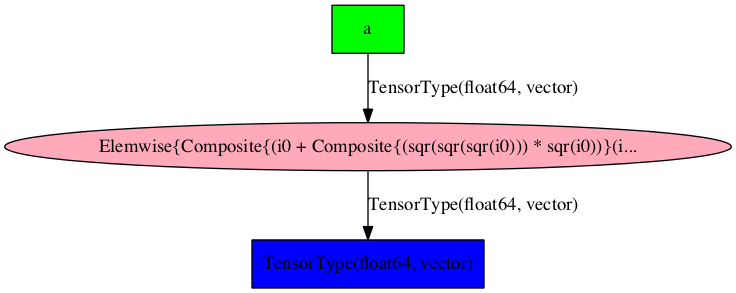
\includegraphics[width=0.35\textwidth]{../hpcs2011_tutorial/pics/f_optimized.png}
%Symbolic programming = *Paradigm shift*: people need to use it to understand it.

\end{frame}


\begin{frame}{Project status?}
  \begin{itemize}
    \item Mature: Theano has been developed and used since January 2008 (6.5 yrs old)
    \item Driven over 100 research papers
    \item Good user documentation
    \item Active mailing list with participants from outside our lab
    \item Core technology for a few Silicon-Valley start-ups
    \item Many contributors (some from outside our lab)
    \item Used to teach many university classes
    \item Has been used for research at Google and Yahoo.
  \end{itemize}
  Theano: \url{deeplearning.net/software/theano/}

  Deep Learning Tutorials: \url{deeplearning.net/tutorial/}
\end{frame}


\section{Pylearn2}
\begin{frame}
  \tableofcontents[currentsection]
\end{frame}

\begin{frame}{Pylearn2 details}
    The core library contains a collection of:
    \begin{itemize}
      \item Training algorithms (e.g. Stochastic and Batch GD, model-specific rules)
      \begin{itemize}
        \item Costs, supervised/unsupervised and exact/estimated (e.g. NLL, Score matching, NCE)
        \item Monitor, history of (functions of) parameters and hyperparameters on different data sets (training, validation, test)
        \item Termination criteria, determine when to stop training
      \end{itemize}
      \item Training extensions, perform actions throughout the training process (e.g., early stopping)
      \item Models (e.g. NNets, ConvNets, RBMs, k-means, PCA, SVMs)
      \item Datasets (e.g. MNIST, CIFAR-10) and preprocessors (LCN, ZCA)
    \end{itemize}
\end{frame}

\begin{frame}{Pylearn2 details, continued}
\begin{itemize}
  \item Data specifications which give semantics to data
  \begin{itemize}
    \item IndexSpace, 1D integer array e.g.\ for labels
    \item VectorSpace, 1D float array e.g.\ for softmax output
    \item Conv2DSpace, 3D float32 arrays e.g.\ for color image input
  \end{itemize}
  \item Allows for automatic conversion when needed e.g.\ labels to one-hot vectors, images to flattened vectors
  \item YAML file allows experiments to be conducted without writing code
\end{itemize}
\end{frame}

\begin{frame}{Project status}
  \begin{itemize}
    \item Has been used for scientific publications, Kaggle competitions, used by many researchers at LISA
    \item Still under rapid development, however the API shouldn't break without warning
    \item Documentation is incomplete, but quickly improving
    \item Features currently in development:
    \begin{itemize}
      \item Recurrent neural networks (RNNs), based on the GroundHog framework developed at LISA
      \item Better hyperparameter search support, using e.g. Hyperopt
    \end{itemize}
  \end{itemize}
\end{frame}

%% \begin{frame}[fragile]
%%   \frametitle{Simple example}

%% % I know it is not Python, but YAML is not supported by listings
%% % close enough? -- PL
%% \lstset{language=python,
%%         commentstyle=\slshape\color{blue},
%%         stringstyle=\color{violet},
%%         basicstyle=\tiny\ttfamily}
%% \begin{lstlisting}
%% !obj:pylearn2.train.Train {
%%     "dataset": !obj:pylearn2.datasets.dense_design_matrix.DenseDesignMatrix &dataset {
%%         "X" : !obj:numpy.random.normal { 'size': [5,3] },
%%     },
%%     "model": !obj:pylearn2.models.autoencoder.DenoisingAutoencoder {
%%         "nvis" : 3,
%%         "nhid" : 4,
%%         "irange" : 0.05,  # Interval from which to sample weights
%%         "corruptor": !obj:pylearn2.corruption.BinomialCorruptor {
%%             "corruption_level": 0.5,
%%         },
%%         "act_enc": "tanh",
%%         "act_dec": null,    # Linear activation on the decoder side.
%%     },
%%     "algorithm": !obj:pylearn2.training_algorithms.sgd.SGD {
%%         "learning_rate" : 1e-3,
%%         "batch_size" : 5,
%%         "monitoring_dataset" : *dataset,
%%         "cost" : !obj:pylearn2.costs.autoencoder.MeanSquaredReconstructionError {},
%%         "termination_criterion" : !obj:pylearn2.termination_criteria.EpochCounter {
%%             "max_epochs": 10,
%%         },
%%     }
%% }
%% \end{lstlisting}
%% \end{frame}

%% \begin{frame}[fragile]
%%   \frametitle{Simple example}

%% \lstset{language=python,
%%         commentstyle=\itshape\color{blue},
%%         stringstyle=\color{violet},
%%         basicstyle=\small
%%         }
%% \begin{lstlisting}
%% # Use Pylearn2 to perform a linear transformation
%% # followed by a softmax
%% x = theano.tensor.vector("x")
%% softmax = pylearn2.models.mlp.Softmax(
%%     n_classes=2, layer_name="softmax", irange=0.05
%% )
%% softmax.set_input_space(
%%   pylearn2.space.VectorSpace(dim=5)
%% )
%% y = softmax.fprop(x)
%% f = theano.function([x], y)
%% print f([0.12, 0.12, 0.43, 0.32, 0.96])
%% # prints [0.43, 0.54]
%% \end{lstlisting}
%% \end{frame}

\section{libgpuarray}
\begin{frame}
  \tableofcontents[currentsection]
\end{frame}

\begin{frame}{libgpuarray: Design Goals}
  \begin{itemize}
  \item Have the base object in C to allow collaboration with more projects.
    \begin{itemize}
    \item We want people from C, C++, ruby, R, \ldots all use the same base GPU ndarray.
    \end{itemize}
  \item Be compatible with CUDA and OpenCL.
  \item Not too simple, (don’t support just matrix).
  \item Support all dtype.
  \item Allow strided views.
  \item But still easy to develop new code that support only a few memory layout.
    \begin{itemize}
    \item This ease the development of new code.
    \end{itemize}
  \end{itemize}
\end{frame}

\begin{frame}{Project status?}
  \begin{itemize}
  \item Usable directly, but not all implementation available.
  \item Multiple GPUs works.
  \item Is the next GPU array container for Theano and is working.
    \begin{itemize}
    \item Not all Theano implementations available now.
    \item OpenCL misses more implementations.
    \item Multiple GPUs on the way.
    \end{itemize}
  \item Web site: \url{http://deeplearning.net/software/libgpuarray/}
  \end{itemize}
\end{frame}

\section{Conclusion}
\begin{frame}
  \tableofcontents[currentsection]
\end{frame}

\begin{frame}{Conclusion}
Theano/Pylearn2/libgpuarry provide an environment for machine learning that is:
\begin{bf}Fast to develop\end{bf}\newline
\begin{bf}Fast to run\end{bf}\newline
\end{frame}

\begin{frame}{Acknowledgments}
\begin{itemize}
\item All people working or having worked at the LISA lab.
\item All Theano/Pylearn 2 users/contributors
\item Compute Canada, RQCHP, NSERC, and Canada Research Chairs for providing funds or access to compute resources.
\end{itemize}
\end{frame}

\begin{frame}
\begin{center}
\Huge
Questions?
\end{center}
\end{frame}


\end{document}
